\chapter{A growing economy in the fluctuating phase}
\label{chap:growing}

The previous chapter left one of the two empirical facts unexplained. A static
Generalized Lotka--Volterra network held at its critical point reproduces the
fat-tailed growth-rate distribution, but it has no stationary size--variance law: the
measured $\sigma(\bar S)$ is a V traced out by the relaxation of an arbitrary initial
condition onto the critical attractor, and once the shape reaches that attractor every
growth rate is exactly zero. The closing remark there was that recovering the slow
size--variance decay seems to need a genuinely nonstationary state, one that keeps
fluctuating rather than relaxing, so that the size-dependent correlations
\citet{moran2024} call for can build up. The natural candidate is the strongly
disordered regime $\sigma > \sigma_c$, where the dynamics on the simplex never settle
but remain chaotic. This is the multiple-attractor or chaotic phase of the disordered
Lotka--Volterra model, studied in the ecological literature
\citep{bunin2017,galla2018,roy2020} and, for the replicator equation to which it maps,
already solved in mean field by \citet{diederich1989}.

Reaching that regime as a model of an economy runs into a different obstacle from the
one of Chapter~\ref{chap:rescaling}. There the total abundance diverged in finite time
and we rescaled time to integrate through the blow-up. Here we want a total that grows
without ever blowing up, an economy whose size increases steadily while its internal
composition keeps churning. The standard model does not provide this: in absolute
variables the chaotic phase still drives a finite-time divergence of $M$. This chapter
makes one change to the model that removes the divergence while keeping the chaos, and
then measures the two firm-growth facts in the resulting state. The size--variance law
is now stationary, and its exponent extrapolates to the empirical value in the
mean-field limit. The fat-tailed growth distribution survives. And both facts disappear
when the disorder is switched off, which locates their origin in the interactions
themselves rather than in any single-firm mechanism.

\section{Relative interactions and steady growth}
\label{sec:relative-model}

The model of Chapter~\ref{chap:rescaling} carries a hidden assumption that an economy
does not share, an absolute scale of size. In \eqref{eq:glv} the self-limitation $-x_i$
would cap an isolated firm at $x_i = 1$, and the interaction term $(Wx)_i$ is quadratic
in the abundances, so the size at which growth, self-limitation and competition balance
is fixed once and for all. A real economy has no such reference size. Its aggregate
output has grown by orders of magnitude over two centuries, while the distribution of
firm sizes and the statistics of their growth have stayed essentially stationary. What
matters to a firm is not its size in absolute terms but its size relative to its
competitors: a company is large or small only by comparison with the rest of the market,
and the same company placed in an economy ten times richer would be in the same
competitive position. The dynamics should therefore be invariant under a rescaling of
the whole economy, $x \to c\,x$, an invariance that \eqref{eq:glv} does not possess,
since its quadratic terms scale differently from its linear one. The finite-time blow-up
of Chapter~\ref{chap:rescaling} is the symptom of this missing invariance: because the
cooperative term grows as $M^2$ while the intrinsic growth is only of order $M$, a
cooperative fluctuation feeds back on itself faster than linearly and reaches infinity
in finite time, which a model with a built-in absolute size cannot avoid.

We restore the invariance by letting the self-limitation and the interactions act on the
abundance of a firm relative to the average firm $m = M/N = \langle x\rangle$ rather than
on its absolute abundance. Keeping the interaction matrix of Chapter~\ref{chap:rescaling},
$W_{ij} = A_{ij}\,\alpha_{ij}$ with $\alpha_{ij} = \mu/C + (\sigma/\sqrt{C})\,z_{ij}$ on
a configuration-model graph, the model becomes
\begin{equation}
    \dot{x}_i = x_i \left( 1 - \frac{x_i}{m} + \frac{(Wx)_i}{m} \right),
    \qquad m = \frac{1}{N}\sum_j x_j .
    \label{eq:relative-glv}
\end{equation}
The only change from \eqref{eq:glv} is the two factors of $1/m$, but it makes the
right-hand side homogeneous of degree one in $x$: under $x \to c\,x$ the mean $m$ scales
in the same way, the ratios $x_i/m$ and $(Wx)_i/m$ are unchanged, and the whole equation
simply rescales, so that if $x(t)$ is a solution then so is $c\,x(t)$. The economy no
longer has a preferred size. The change is also the economically natural one: a
competitor's pressure on firm $i$ is now set by its market share $x_j/m$ rather than by
its absolute size, and a firm's own crowding is measured against the typical firm rather
than against a fixed ceiling, so what drives the dynamics is relative standing in the
market, as it should be. The intrinsic Malthusian rate $1$ is left untouched and remains
the engine of growth, while the interactions, now made relative, only regulate it. We
operate at a competitive mean $\mu$ and at a disorder $\sigma$ above the chaotic
threshold $\sigma_c = \sqrt{2}$ \citep{diederich1989}; the operating point is specified
with the measurements below.

The same point appears formally in the equation for the total. Writing $x_i = M y_i$
with $y$ on the simplex, and using the shorthands of Chapter~\ref{chap:rescaling}, the
sum of \eqref{eq:relative-glv} over $i$ gives
\begin{equation}
    \dot{M} = M \left[\, 1 + N\big( y^{\!\top} W y - y^{\!\top} y \big)\,\right]
            \equiv M\, g_{\mathrm{eff}}(y),
    \label{eq:Mdot-relative}
\end{equation}
where the right-hand side of the absolute model \eqref{eq:app-Mdot} instead carried a
term in $M^2$, the quadratic feedback responsible for the finite-time singularity.
Dividing the interactions by $m$ removes one power of $M$: the quadratic term becomes
linear, and \eqref{eq:Mdot-relative} is the equation of plain exponential growth,
$M(t) \sim e^{g_{\mathrm{eff}} t}$, with no singularity. In the operating regime
$g_{\mathrm{eff}}$ settles to a small positive constant, so the economy grows at a steady
rate over unbounded physical time.

The shape obeys, again from \eqref{eq:relative-glv} and the quotient rule,
\begin{equation}
    \dot{y}_i = y_i \left( f_i - \langle f \rangle \right),
    \qquad f_i = 1 - N y_i + N (Wy)_i,
    \qquad \langle f \rangle = \sum_j y_j f_j = g_{\mathrm{eff}},
    \label{eq:replicator}
\end{equation}
which is a replicator equation with the linear fitness $f$, the canonical description of
frequency-dependent selection, in which a firm gains share precisely when its fitness
exceeds the market average $\langle f \rangle$, and is exactly the correspondence between
Lotka--Volterra and replicator dynamics used in Chapter~\ref{chap:rescaling}
\citep{hofbauer81}. Two features distinguish
\eqref{eq:replicator} from the rescaled dynamics of that chapter. First, it is written
in physical time $t$, not in a stretched time $\tau$: because the relative model does
not blow up, no time rescaling is needed, and $M(t)$ grows exponentially in the same
$t$ in which the firms are observed. Second, in the disordered regime $\sigma > \sigma_c$
the replicator flow \eqref{eq:replicator} does not relax to a fixed point but remains
chaotic, so the growth rates $\dot y_i / y_i = f_i - \langle f\rangle$ never vanish.
This is the persistently fluctuating state the previous chapter identified as the
missing ingredient. As in the literature \citep{bunin2017,roy2020} we add a small
immigration term that pulls each share gently toward $1/N$, which sets a floor of rarity
and prevents firms from reaching exact extinction; we use a rate $\lambda = 10^{-3}$.

We integrate \eqref{eq:replicator} together with $\mathrm{d}\ln M/\mathrm{d}t =
g_{\mathrm{eff}}$ directly in physical time. The shape stays on the bounded simplex and
the scale is tracked in logarithm, so nothing overflows however large $M$ becomes. We
use an explicit Runge--Kutta solver throughout: at the system sizes reached below
($N$ up to $1.3\times10^4$) the implicit solvers tried first switched to a dense
Jacobian and became prohibitively slow, whereas the explicit method integrates one run
to $t = 250$ in about ten seconds at $N = 10^4$.

Before turning to the firm-growth statistics it helps to see where in parameter space
this fluctuating, growing state lives. Figure~\ref{fig:phase-diagram} maps the behaviour
of \eqref{eq:relative-glv} over the plane of the mean interaction $\mu$ and the disorder
$\sigma$, classified from the late-time dynamics of many graph realizations. Two genuine
transitions organize it. The dynamical threshold $\sigma_c = \sqrt{2}$ separates a frozen
regime below, where the shape relaxes to a fixed point and the growth rates vanish, from
the chaotic regime above, where it never settles. Cutting across it, the line
$g_{\mathrm{eff}} = 0$ separates a growing economy from a shrinking one. Where the
competition is strong and the disorder high, coexistence collapses and the dynamics
either condense onto a few firms or grow explosively. The firm-growth statistics of this
chapter belong to the chaotic, growing band, the wedge bounded below by $\sigma_c$, on
one side by the $g_{\mathrm{eff}} = 0$ line, and on the other by the condensed corner.
The key point is that this is an extended region rather than an isolated point: the model
reproduces the empirical facts across a band of parameters, so what follows describes the
behaviour of the model and not a single tuned operating point.

\begin{figure}[htbp]
    \centering
    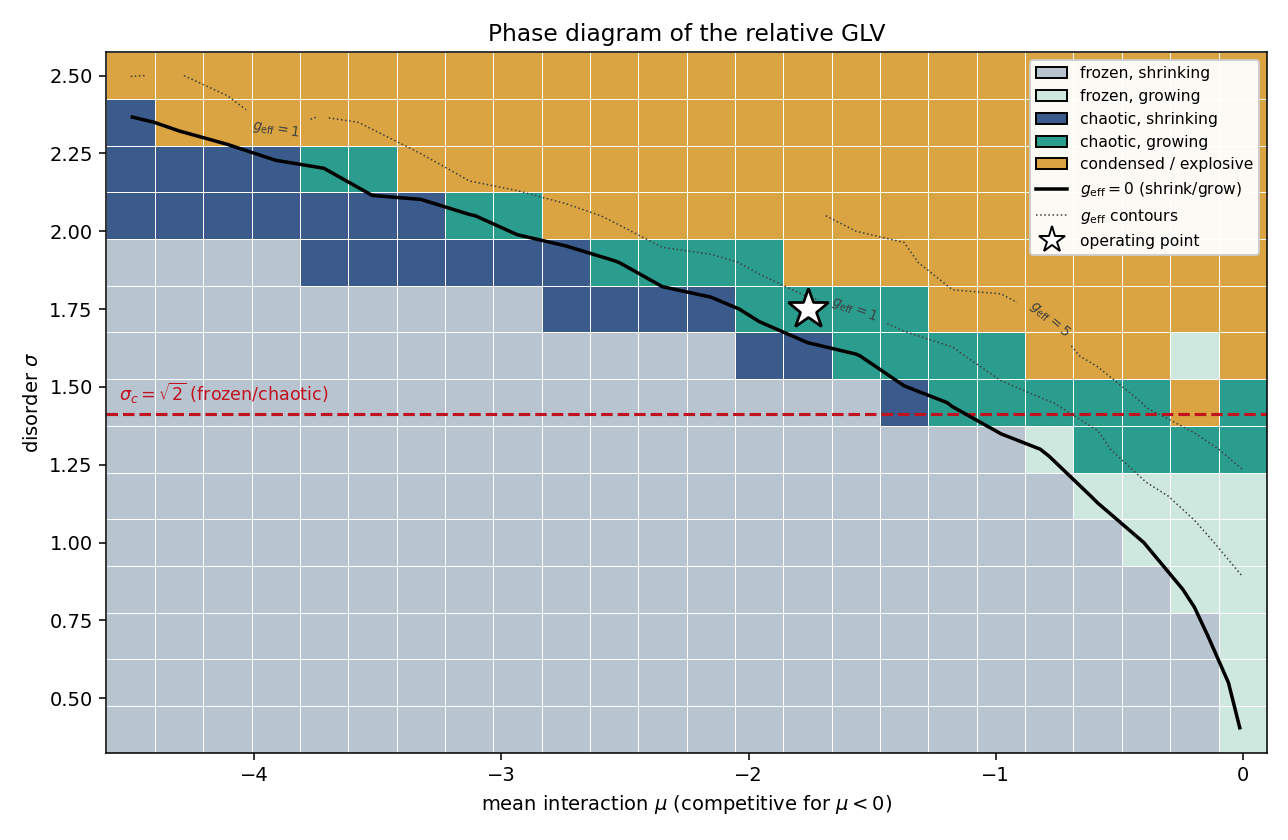
\includegraphics[width=\linewidth]{phase_diagram.png}
    \caption{Phase diagram of the relative model \eqref{eq:relative-glv} over the mean
    interaction $\mu$ (competitive for $\mu < 0$) and the disorder $\sigma$, classified
    from the late-time dynamics ($N = 4000$, fifteen realizations per cell). Below
    $\sigma_c = \sqrt{2}$ (red dashed) the shape relaxes and nothing fluctuates; above it
    the dynamics are chaotic. The solid line is the growth boundary
    $g_{\mathrm{eff}} = 0$, with $g_{\mathrm{eff}}$ magnitude contours dotted. The
    firm-growth statistics are measured in the chaotic, growing band (teal), bounded by
    $\sigma_c$, the $g_{\mathrm{eff}} = 0$ line, and the condensed or explosive corner.
    The band is an extended region, not a single point.}
    \label{fig:phase-diagram}
\end{figure}

Figure~\ref{fig:growing-churn} shows a single run in this regime. The total abundance
(left) climbs as a straight line in $\log M$ over the whole integration, the steady
exponential growth of \eqref{eq:Mdot-relative}, with no sign of a blow-up. The relative
firm sizes $S_i = N y_i$ (right) do not settle: after an initial transient they keep
exchanging rank and spanning orders of magnitude, the persistent chaos of the
$\sigma > \sigma_c$ phase. The economy grows while its composition keeps turning over.

\begin{figure}[htbp]
    \centering
    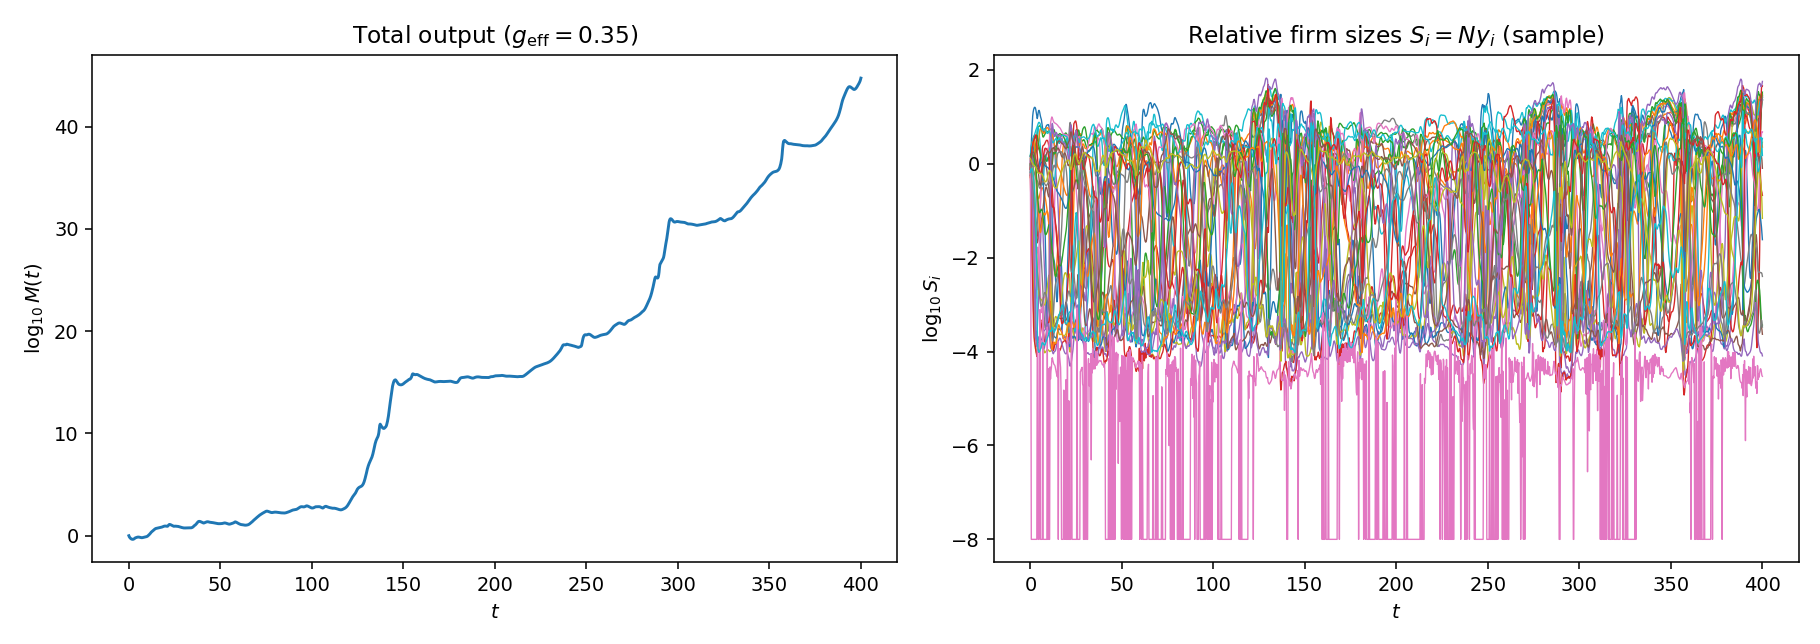
\includegraphics[width=\linewidth]{growing_growth_churn.png}
    \caption{A single run of the relative model \eqref{eq:relative-glv} at $\mu = -1.76$,
    $\sigma = 1.75$, $\lambda = 10^{-3}$ on a power-law graph with $N = 6400$. Left: the
    total abundance grows exponentially in physical time, $\log_{10} M(t)$ rising
    linearly, with no finite-time divergence. Right: a sample of relative firm sizes
    $S_i = N y_i$, which keep fluctuating and exchanging rank rather than relaxing to a
    fixed point.}
    \label{fig:growing-churn}
\end{figure}

\section{Firm-growth statistics in the fluctuating state}
\label{sec:growing-observables}

We measure the two firm-growth facts on the relative sizes $S_i = N y_i$, whose
cross-sectional mean is one by construction. The common growth of the economy is divided
out in the same step, since $\ln S_i = \ln x_i - \ln M + \ln N$, so the size and its
growth $g_i = \Delta \ln S_i$ are the idiosyncratic part of a firm's trajectory, exactly
what the data measure. We follow the empirical protocol: each firm contributes while it
is listed, that is while $S_i$ stays above the immigration floor, and we read growth
rates over a fixed yearly horizon $\Delta t$ rather than the solver's adaptive one. All
statistics are taken in a late window, after the initial relaxation has passed, and
restricted to firms that persist across it.

Two cautions, both inherited from the previous chapters, shape the measurement. The
volatility per firm is $\sigma_i = \sqrt{\pi/2}\,\langle |g_i - \langle g_i\rangle|
\rangle$, a mean-absolute-deviation estimator robust to the fat tails. And the
size--volatility relation is fitted only where it is a power law: a small immigration
floor makes the smallest firms quiet, producing a plateau at the bottom of the size
range, so we fit the decline above the plateau and report the coefficient of
determination $R^2$ of that fit, rather than forcing a single slope across a shape that
is not a power law.

Figure~\ref{fig:growing-msb} shows both observables at the operating point
$\mu = -1.76$, $\sigma = 1.75$ marked in Figure~\ref{fig:phase-diagram}, in the
stationary fluctuating state. The size--volatility relation (left) now falls
monotonically over the fitted range, $\sigma(\bar S) \sim \bar S^{-\beta}$ with a clean
power law ($R^2 \approx 0.98$ in the economy shown), in contrast to the rising V of
Chapter~\ref{chap:results}: large firms are now less volatile than small ones, as in the
data. The growth-rate distribution (right) is
sharply peaked and fat-tailed, with both flanks heavier than the Laplace reference and
no systematic asymmetry between them. The two facts that the static critical model could
not deliver together, a monotone size--volatility decay and a symmetric fat-tailed tent,
are both present here, and both are stationary properties of the chaotic state rather
than transients of a relaxation.

\begin{figure}[htbp]
    \centering
    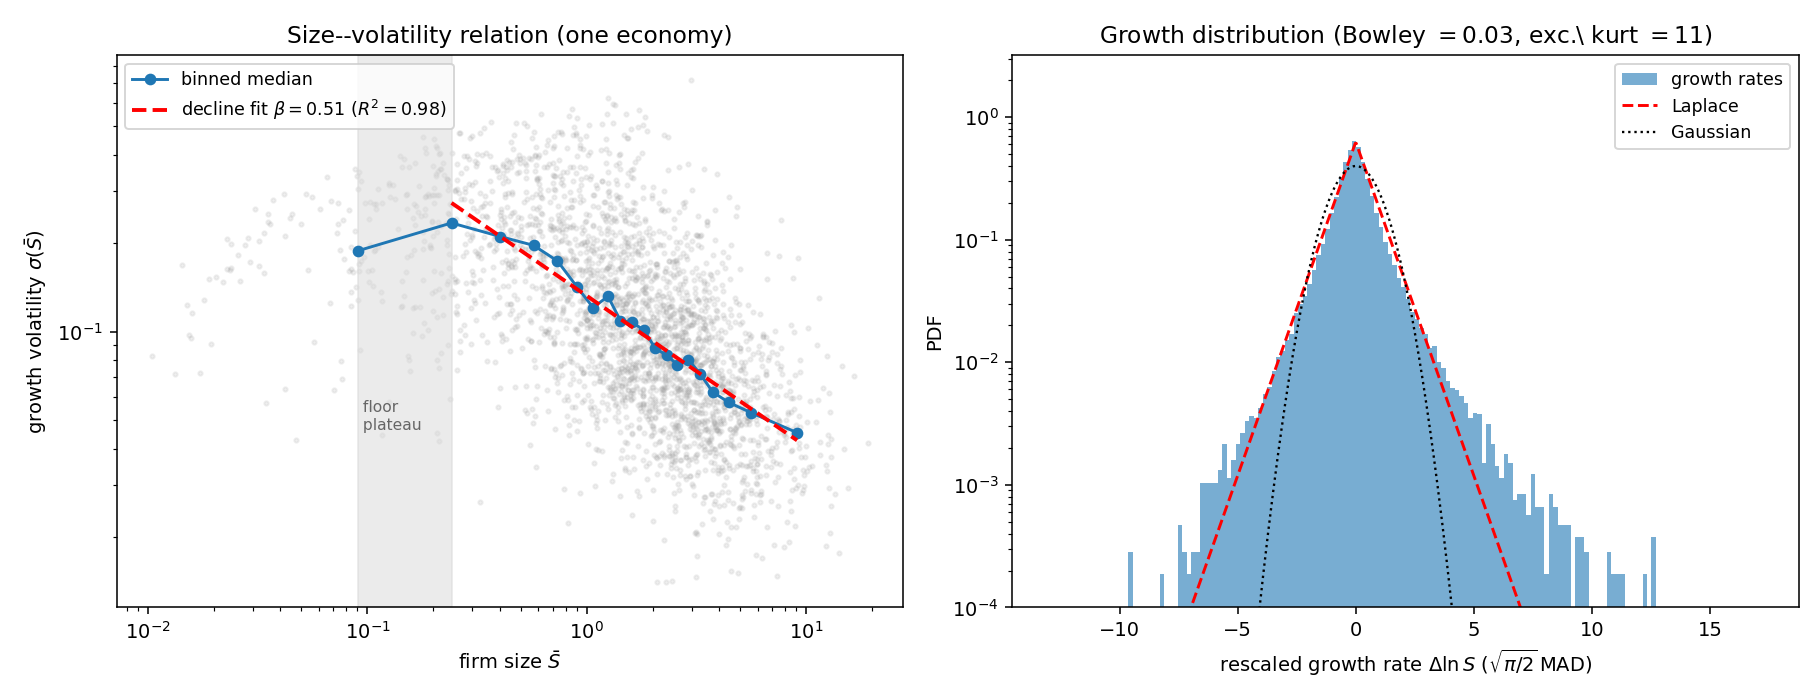
\includegraphics[width=\linewidth]{growing_stationary_msb.png}
    \caption{Firm-growth statistics at $\mu = -1.76$, $\sigma = 1.75$. Left: the
    size--volatility relation in a single economy ($N = 6400$); volatility falls as a
    power law over the fitted decline above the small-firm immigration-floor plateau
    (shaded), here with exponent $\beta \approx 0.5$ and $R^2 = 0.98$. Right: the
    growth-rate distribution pooled over economies, sharply peaked and fat-tailed,
    heavier than the Laplace reference on both flanks and close to symmetric
    (Bowley $\approx 0$), far above the Gaussian.}
    \label{fig:growing-msb}
\end{figure}

\section{Finite size and the mean-field limit}
\label{sec:growing-finite-size}

The chaotic state above is not equally robust at all system sizes, and the way it
strengthens with $N$ both validates the measurement and fixes the value of the
size--variance exponent. At small $N$ the persistent chaos is fragile: for many graph
realizations the shape, after fluctuating for a while, eventually collapses onto a fixed
point and freezes, recovering the relaxation transient of Chapter~\ref{chap:results}.
This is the known finite-size metastability of the fluctuating phase
\citep{roy2020}: rare large excursions drive firms below the floor, and the state can
fall into a frozen attractor. Figure~\ref{fig:growing-trajectories} contrasts the two
outcomes directly, a realization that freezes onto a fixed point against one that keeps
churning to the end of the run. Measuring in a short early window, as one is
tempted to do, reports the firms while they still fluctuate and so mistakes the frozen
transient for a stationary state; only integrating to long times separates the two.

\begin{figure}[htbp]
    \centering
    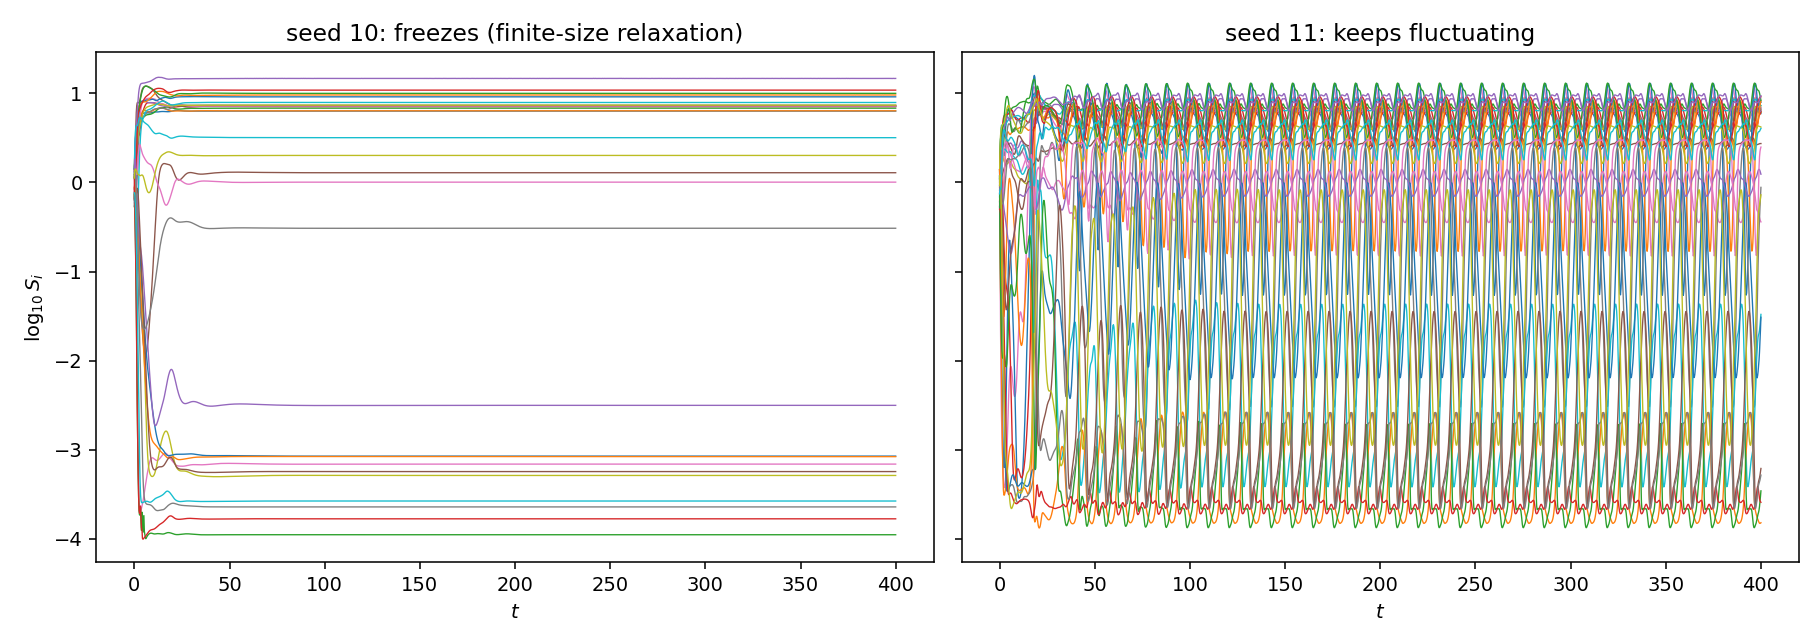
\includegraphics[width=\linewidth]{growing_trajectories.png}
    \caption{Two finite-size realizations at $N = 600$, $\mu = -1.76$, $\sigma = 1.75$.
    Left: the shares churn for a while and then freeze onto a fixed point, the
    finite-size relaxation transient. Right: a realization in which the chaos persists
    for the whole run. Whether a given realization freezes or keeps fluctuating is a
    finite-size accident that becomes rarer as $N$ grows.}
    \label{fig:growing-trajectories}
\end{figure}

Whether a realization freezes or keeps fluctuating is a finite-size accident that
becomes rarer as $N$ grows. The left panel of Figure~\ref{fig:growing-meanfield}
records the fraction of realizations that remain persistently chaotic at long times: it
is fragile at small $N$, with half to three-quarters of realizations persisting, and
reaches all of them by $N \approx 6000$. The fragility is
a finite-size effect; in the mean-field limit the fluctuating phase is the generic
outcome of the operating regime, consistent with the dynamical mean-field picture of
\citet{bunin2017} and \citet{roy2020}.

The same limit fixes the size--variance exponent. Measured on the persistent
realizations, $\beta$ falls steadily with system size, from about $0.68$ at $N = 800$
toward $0.25$ at $N = 1.3\times10^4$ (Fig.~\ref{fig:growing-meanfield}, right). The
finite-size correction is the natural Gaussian one, of order $N^{-1/2}$, and a fit of
$\beta(N) = \beta_\infty + c\,N^{-1/2}$ extrapolates to
\begin{equation}
    \beta_\infty \approx 0.17
    \label{eq:beta-infinity}
\end{equation}
in the mean-field limit (Fig.~\ref{fig:growing-betainf}). This value lies inside the
empirical band $\beta \approx 0.15$--$0.20$. The relative model therefore reproduces not only the
sign of the size--variance relation but, within the uncertainty of the extrapolation,
its exponent: the slow size--variance decay that the static critical model could not
supply emerges here as a stationary law with the right magnitude.

\begin{figure}[htbp]
    \centering
    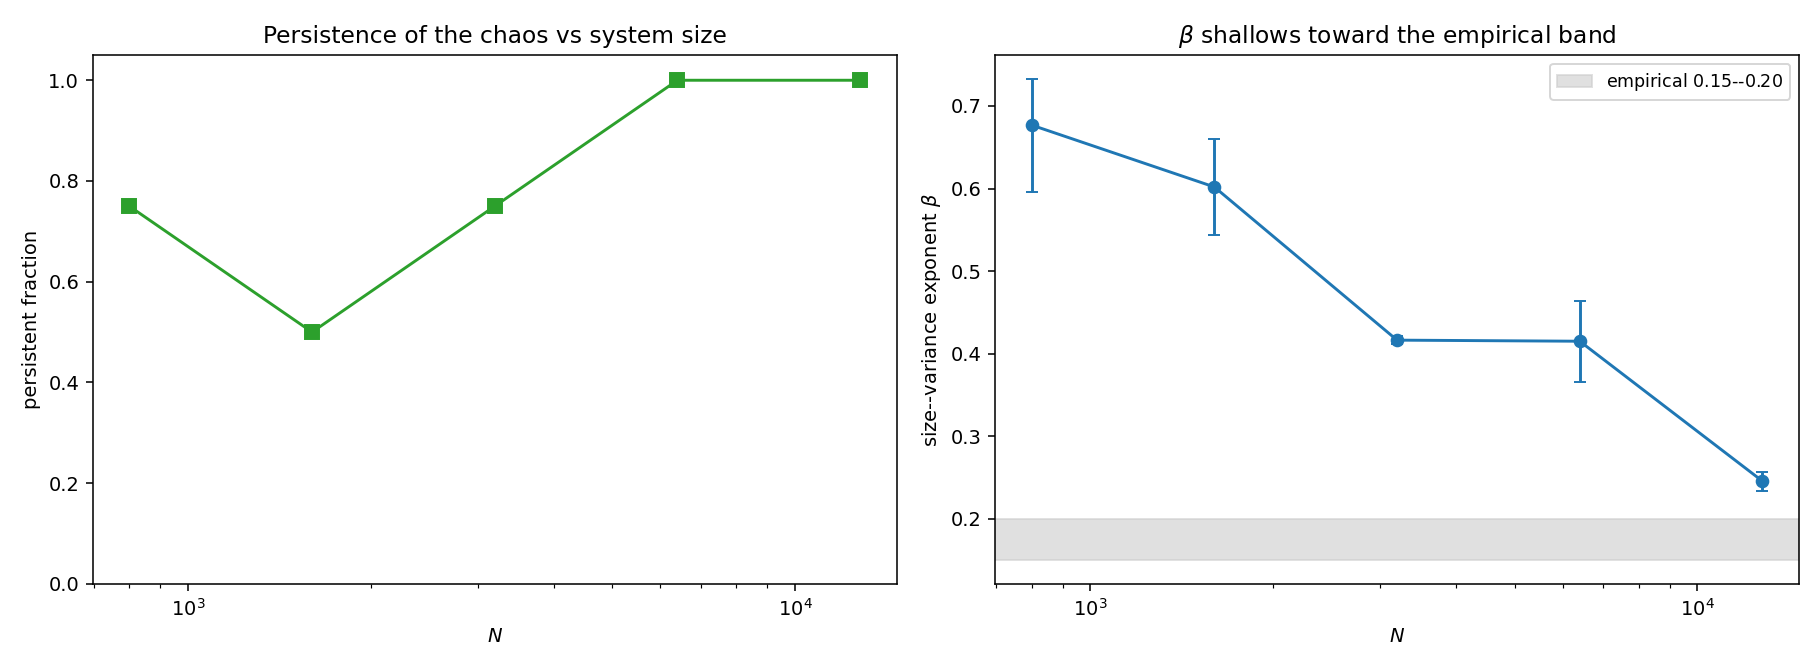
\includegraphics[width=\linewidth]{growing_meanfield.png}
    \caption{Approach to the mean-field limit at $\mu = -1.76$, $\sigma = 1.75$,
    $\lambda = 10^{-3}$. Left: the fraction of realizations that stay persistently
    chaotic at long times rises to one by $N \approx 6000$, so the finite-size
    fragility of the fluctuating phase is a finite-$N$ effect. Right: the
    size--variance exponent $\beta$ measured on the persistent realizations falls
    toward the empirical band (shaded) as $N$ grows.}
    \label{fig:growing-meanfield}
\end{figure}

\begin{figure}[h]
    \centering
    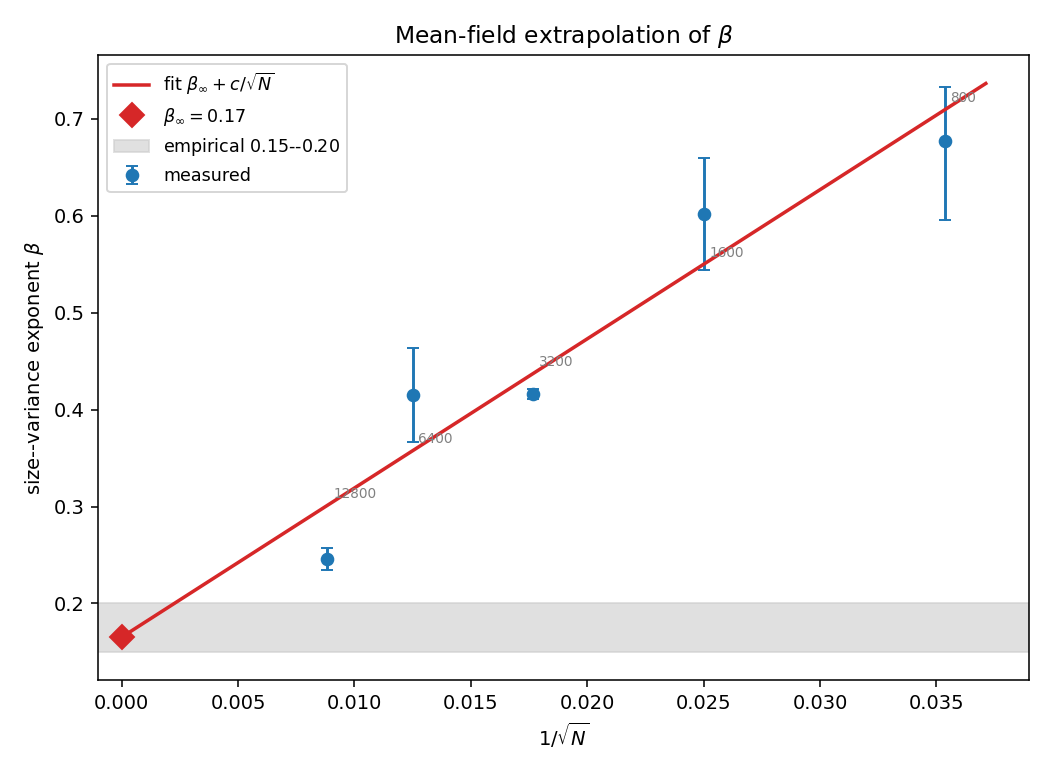
\includegraphics[width=0.78\linewidth]{growing_beta_extrapolation.png}
    \caption{Extrapolation of the size--variance exponent to the mean-field limit.
    Measured $\beta$ against $N^{-1/2}$, with a linear fit. The intercept gives
    $\beta_\infty \approx 0.17$, inside the empirical band
    $\beta \approx 0.15$--$0.20$ (shaded). Error bars are the interquartile spread over
    graph realizations.}
    \label{fig:growing-betainf}
\end{figure}

\section{The role of the interactions}
\label{sec:growing-ablation}

The model carries no external heterogeneity and no explicit noise: the only source of
fluctuation is the disordered interaction matrix. To confirm that the firm-growth
statistics are produced by the interactions, and are not an artifact of the
multiplicative structure or the immigration floor, we switch the disorder off and dial
it back up. Table~\ref{tab:growing-ablation} sweeps $\sigma$ at fixed $\mu$, $\lambda$
and $N$. Below the threshold $\sigma_c = \sqrt{2}$ the dynamics freeze: the late-time
growth fluctuations are zero to the precision quoted, the shape has relaxed to a fixed
point, and there is no fluctuating state to measure. The persistent fluctuations and
the fat-tailed tent appear only once $\sigma$ crosses $\sigma_c$, growing with the
disorder. With no noise in the model, the fluctuations can come only from the disorder,
and removing it removes them entirely.

\begin{table}[h]
    \centering
    \begin{tabular}{rccc}
        \hline
        $\sigma$ & growth fluctuation & excess kurtosis & fat-tailed tent? \\
        \hline
        $0.00$ & $0.000$ & --   & no  \\
        $0.50$ & $0.000$ & --   & no  \\
        $1.00$ & $0.000$ & --   & no  \\
        $1.41$ & $0.000$ & --   & no  \\
        $1.60$ & $0.085$ & $14$ & yes \\
        $1.75$ & $0.175$ & $14$ & yes \\
        \hline
    \end{tabular}
    \caption{Disorder ablation at $\mu = -1.76$, $\lambda = 10^{-3}$, $N = 3200$ on a
    power-law graph. ``Growth fluctuation'' is the standard deviation of the pooled
    late-window growth rates. Below the chaotic threshold $\sigma_c = \sqrt{2}$ the state
    freezes (growth fluctuation zero to the precision quoted) and there is no genuine
    fluctuating distribution to characterize, so the kurtosis is left blank; the
    persistent fluctuations and the fat-tailed tent switch on only once $\sigma$ crosses
    $\sigma_c$. (A nonzero $\beta$ can still be fitted below threshold, but on a frozen
    state during its relaxation, the V transient of Chapter~\ref{chap:results}, not on a
    stationary fluctuating law.)}
    \label{tab:growing-ablation}
\end{table}

This is the distinction the introduction asked for. The firm-growth statistics here are
a between-firm effect, generated by the network of interactions, and not a within-firm
one: with the interactions removed there is nothing left, no noise carrying the
fluctuations and no single-firm mechanism producing a tail. It is also the size of the
result that separates this model from the simplest alternatives. A growing economy with
a stationary heavy-tailed size distribution can be had from a mean-field multiplicative
model with injected noise \citep{bouchaudmezard2000}, but there the fluctuations are put
in by hand and there is no network. Here the same growing aggregate, the heavy tails,
and the slow size--variance decay arise together from a single ingredient, the disordered
interactions, which is the size-dependent correlation mechanism \citet{moran2024}
identify as the one the granular models lack.

\section{Discussion}
\label{sec:growing-discussion}

This chapter closes the gap left by Chapter~\ref{chap:results}. Making the
Lotka--Volterra interactions relative to the mean firm turns the finite-time divergence
of the standard model into steady exponential growth, and in the disordered regime
$\sigma > \sigma_c$ the resulting economy grows while its composition fluctuates without
ever settling. In this genuinely nonstationary state the size--variance relation is a
stationary law that falls monotonically with the empirical sign, and its exponent
extrapolates to $\beta_\infty \approx 0.17$ in the mean-field limit, inside the empirical
band; the growth-rate distribution is symmetric and fat-tailed; and switching off
the disorder removes both, locating their origin in the interactions.

Four honest qualifications bound the claim. The model itself is not new: it is the
disordered replicator equation \citep{diederich1989,hofbauer81}, equivalently the
chaotic phase of the disordered Lotka--Volterra model \citep{bunin2017,galla2018,roy2020},
and its finite-size fragility and approach to a robust mean-field fluctuating phase are
known features of that system. What is specific here is the use of this state, on a
heterogeneous graph and with the interactions made relative so that the aggregate grows,
as a model of firm growth, and the finding that its firm-growth statistics match the
empirical ones. The extrapolated exponent, second, lands inside the empirical band but is
not sharply pinned: the largest-$N$ points are the noisiest, and tightening the estimate
would need more realizations at $N \gtrsim 10^4$. Third, the economy grows in the large
majority of realizations rather than in every one, the operating point sitting in the
growing band but not far from its $g_{\mathrm{eff}} = 0$ boundary. Finally, the match is in the marginal facts, the size--variance exponent and
the shape of the growth distribution; showing directly that the disordered interactions
produce the size-dependent correlation structure of \citet{moran2024}, rather than only
its consequences, is the natural next step and is left to future work.
